\chapter{Results}

The results gathered are from a randomly initialized RNN on the data set MNIST. The MNIST data set consists of $28 \times 28$ pixel handwritten digit images. The task is to classify the images into $10$ digit classes. For the RNN, the image is sequentially fed into the RNN, here $28$ pixels at a time. 

The input and ouput dimensions decide the architecture of the RNN. The input layer then consists of $28$ nodes, the output $10$. The hidden layer size is variable and initial sizes are set. The weights are randomly initialized for the symmetry break, and biases are left at zero. 

The MNIST data set is divided into mini-batches. A mini-batch consists of $1000$ samples, as the HF relies on bigger mini-batches. An epoch is a complete progression of mini-batches through the entire data set, of which there are in total $60 000$. Of the entire set, however, a selection set of $10 000$ samples was used, making the training set $50000$. A total of $11$ epochs was performed on one training run. Finally, a separate test set of $10000$ samples benchmarked the RNN. The initialization is omitted from the results, consisting of the first epoch, $50$ mini-batches. The omittance is to resolve the more important training part better.

The activation for the hidden layer $a_h(x) = 1/(1 + e^{-x})$ is the sigmoid. The output or output activation \[a_o(z_j) = \frac{e^{z_j}}{\sum_{k=1}^N e^{z_k}}\] is the softmax function. Accordingly the "matching" cost or energy function is the cross-entropy function \[C(z,x) = - \sum_i [x_i] \log [\hat{x}]_i\] where $\hat{x} = a_o(z)$ is the models prediction and $x$ is the target. Using one-hot encoding the target $x$ is a vector of zeroes except at one location. The "matching" property leads to \[\nabla_z C(z,x) = \hat{x} - x \text{ and } H_{C(z,x)} = \text{diag}(\hat{x}) - \hat{x} \hat{x}^\top\] which is left as an exercise but what can be seen is a benign Hessian independent of the target. 

For the changes in the RNN, a relaxation function $e(5/(2n)) - 1$ where $n$ is the current epoch, was used to regulate changes and make them less probable as the training progresses. To this a uniform random number $r$ is drawn and if smaller $ r < e(5/(2n)) - 1$ the perturbation will proceed.

\section{Sizes and Plots}

Different initial sizes of the hidden layer were studied, comparing with and without the regularization for each size. The sizes were $L_h = 27, 37, 47, 57, 67$, from which the training started. However, the RNNs sizes with regularization changed throughout the training. How this happened is ignored as the moves are incomparable; removing a weight vs. a node is an altogether different change, and all the moves are treated without bias in the algorithm. 

In the below plots, w in the legends stands for with the algorithm. 

\begin{figure}[h]
    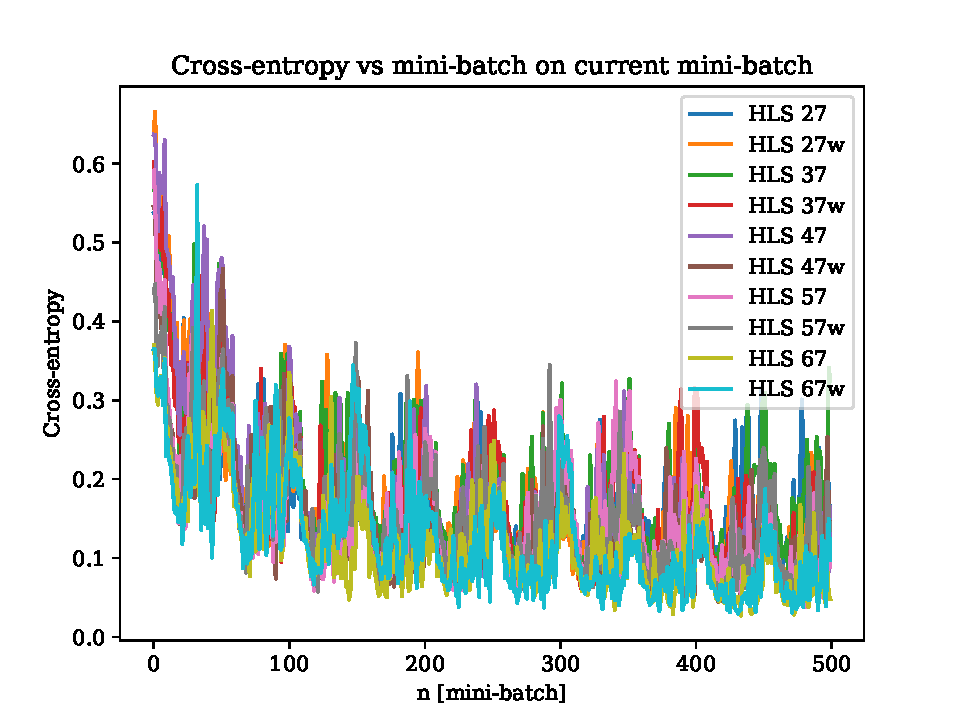
\includegraphics[width = \textwidth]{imgs/ps.pdf}
    \caption{Cross-entropy plot on the mini-batch for various initial sizes of the RNN, omitting first epoch. With and without the algorithm.}
    \label[fig]{E}
\end{figure}

\begin{figure}[h]
    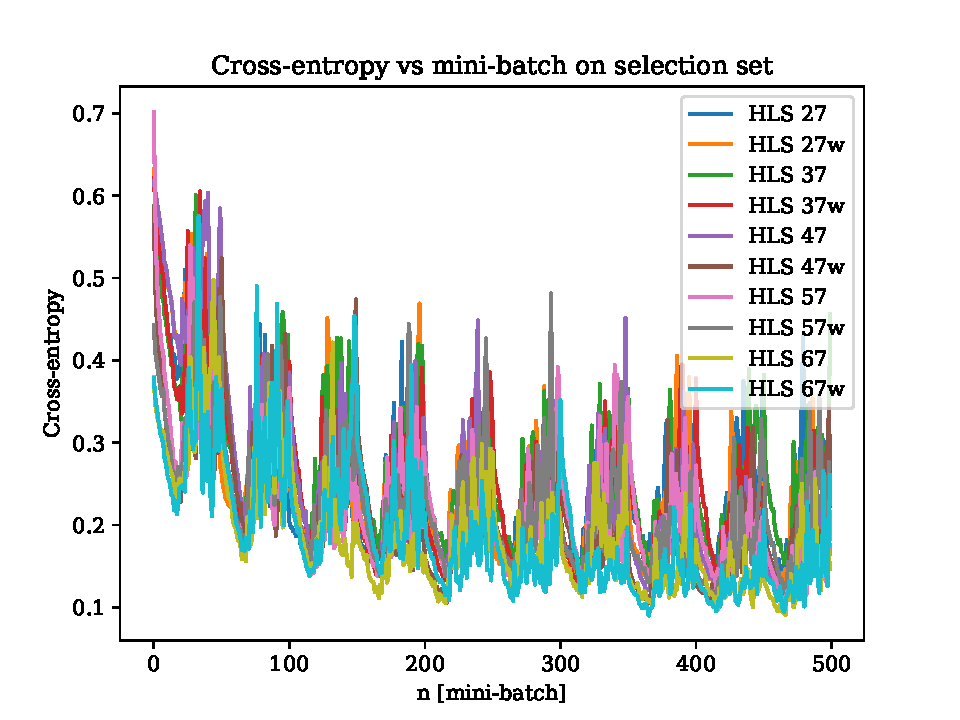
\includegraphics[width = \textwidth]{imgs/ps1.pdf}
    \caption{Cross-entropy plot on the selection set for various initial sizes of the RNN, omitting first epoch. With and without the algorithm.}
    \label[fig]{E_sel}
\end{figure}

As can be seen, a plot of energy during training. \ref{E} on the current mini-batch and \ref{E_sel} on the selection set. The variation is due to the mini-batch being a small subset.

\begin{figure}[h]
    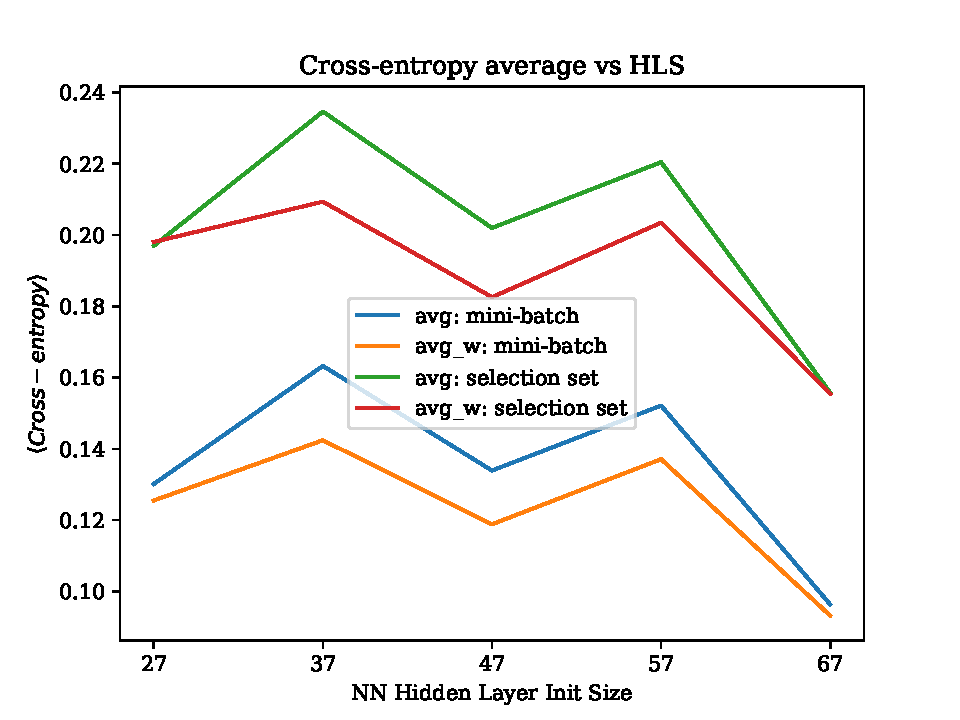
\includegraphics[width = \textwidth]{imgs/ps2.pdf}
    \caption{Average cross-entropy across training, after the first four epochs. For the mini-batch and sel, selection set. With and without the algorithm.}
    \label[fig]{avg}
\end{figure}

\begin{figure}[h]
    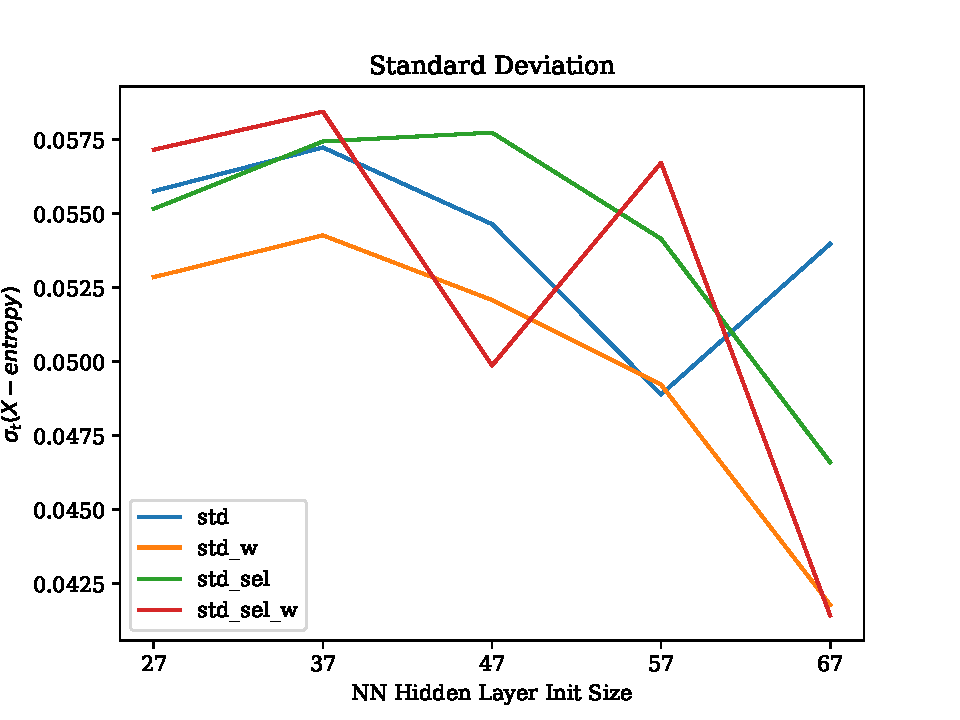
\includegraphics[width = \textwidth]{imgs/ps3.pdf}
    \caption{Standard deviation of the cross entropy across training, after the first four epochs. For the mini-batch and sel, selection set. With and without the algorithm.}
    \label[fig]{std}
\end{figure}

In the plots of the average \ref{avg} and standard deviation \ref{std}, a clear difference with or without the algorithm in the average which was stable. However, the standard deviation varied greatly depending on the number of epochs included in the calculation; this is due to randomly generated mini-batches.  

\begin{figure}[h]
    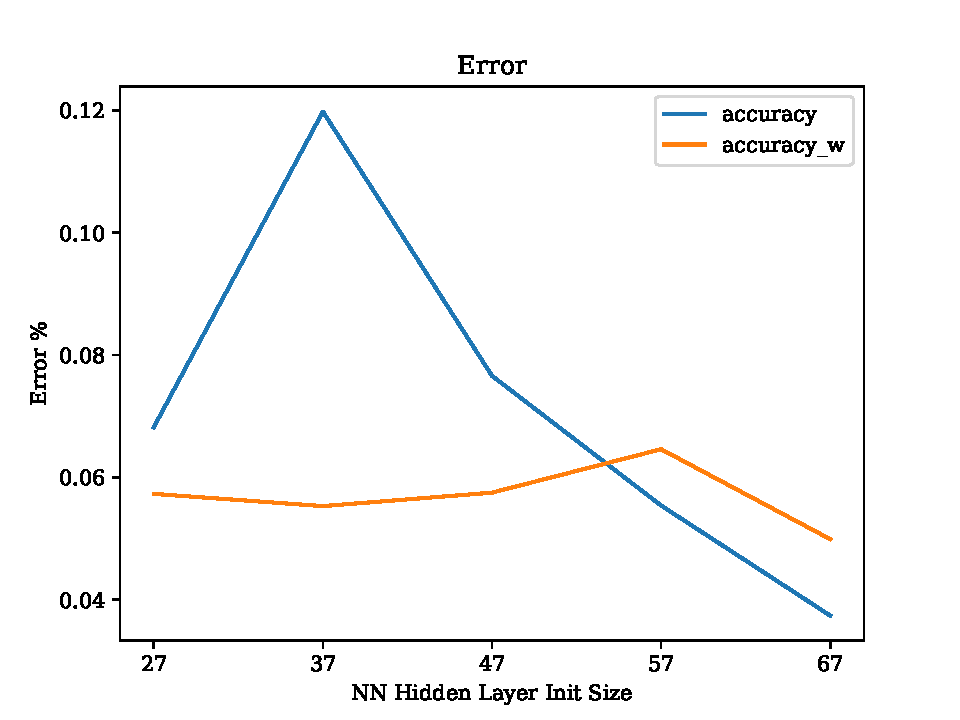
\includegraphics[width = \textwidth]{imgs/ps4.pdf}
    \caption{Error on test set, with and without the algorithm.}
    \label[fig]{acc}
\end{figure}

The last plot of the error on the test set \ref{acc} with and without the algorithm, which seems to perform well for small to medium-sized NNs.

\begin{table}[h]
    \centering
    \begin{tabular}{|l|l|l|l|l|l|}
    \hline
       Hidden Layer Size & 27 & 37 & 47 & 57 & 67 \\
    \hline
       - & 6.82 & 11.98 & 7.66 & 5.54 & 3.74 \\
    \hline
       w & 5.73 & 5.53 & 5.75 & 6.46 & 4.99 \\
    \hline
    \end{tabular}
    \caption{Error in \%, with and without the algorithm.}
    \label[table]{acc_t}
\end{table}

In the table \ref{acc_t}, the error can be seen in plain text, w for with the regularization.
